% vim:ft=tex
% rubber: module xelatex

\subsection{Camera calibration}
\label{sec:calibration}

For the camera calibration part of the application, we have
implemented the calibration algorithm from \cite{TSAI}, a
classic and often-cited calibration method. The article encompasses
several different methods of calibration; we are implementing the
method that the article describes as ``the monoview non-coplanar
case''. That is, the calibration is performed from a single image
of a calibration object that has calibration points in several (world) planes.

The calibration object we used can be seen in figure~\ref{fig:calib-object}.
It consists of two adjacent faces of a cube, the left face having 35 regularly-spaced circular calibration points,
and the right face 28 such points. The distance between point centres is 1.5
inches. The world coordinate system is chosen to be a right-handed
coordinate system, centred at the bottom corned of the cube, so the
left face corresponds to the YZ plane, and the right face corresponds
to the XZ plane.

\begin{figure}[h]
  \centering
  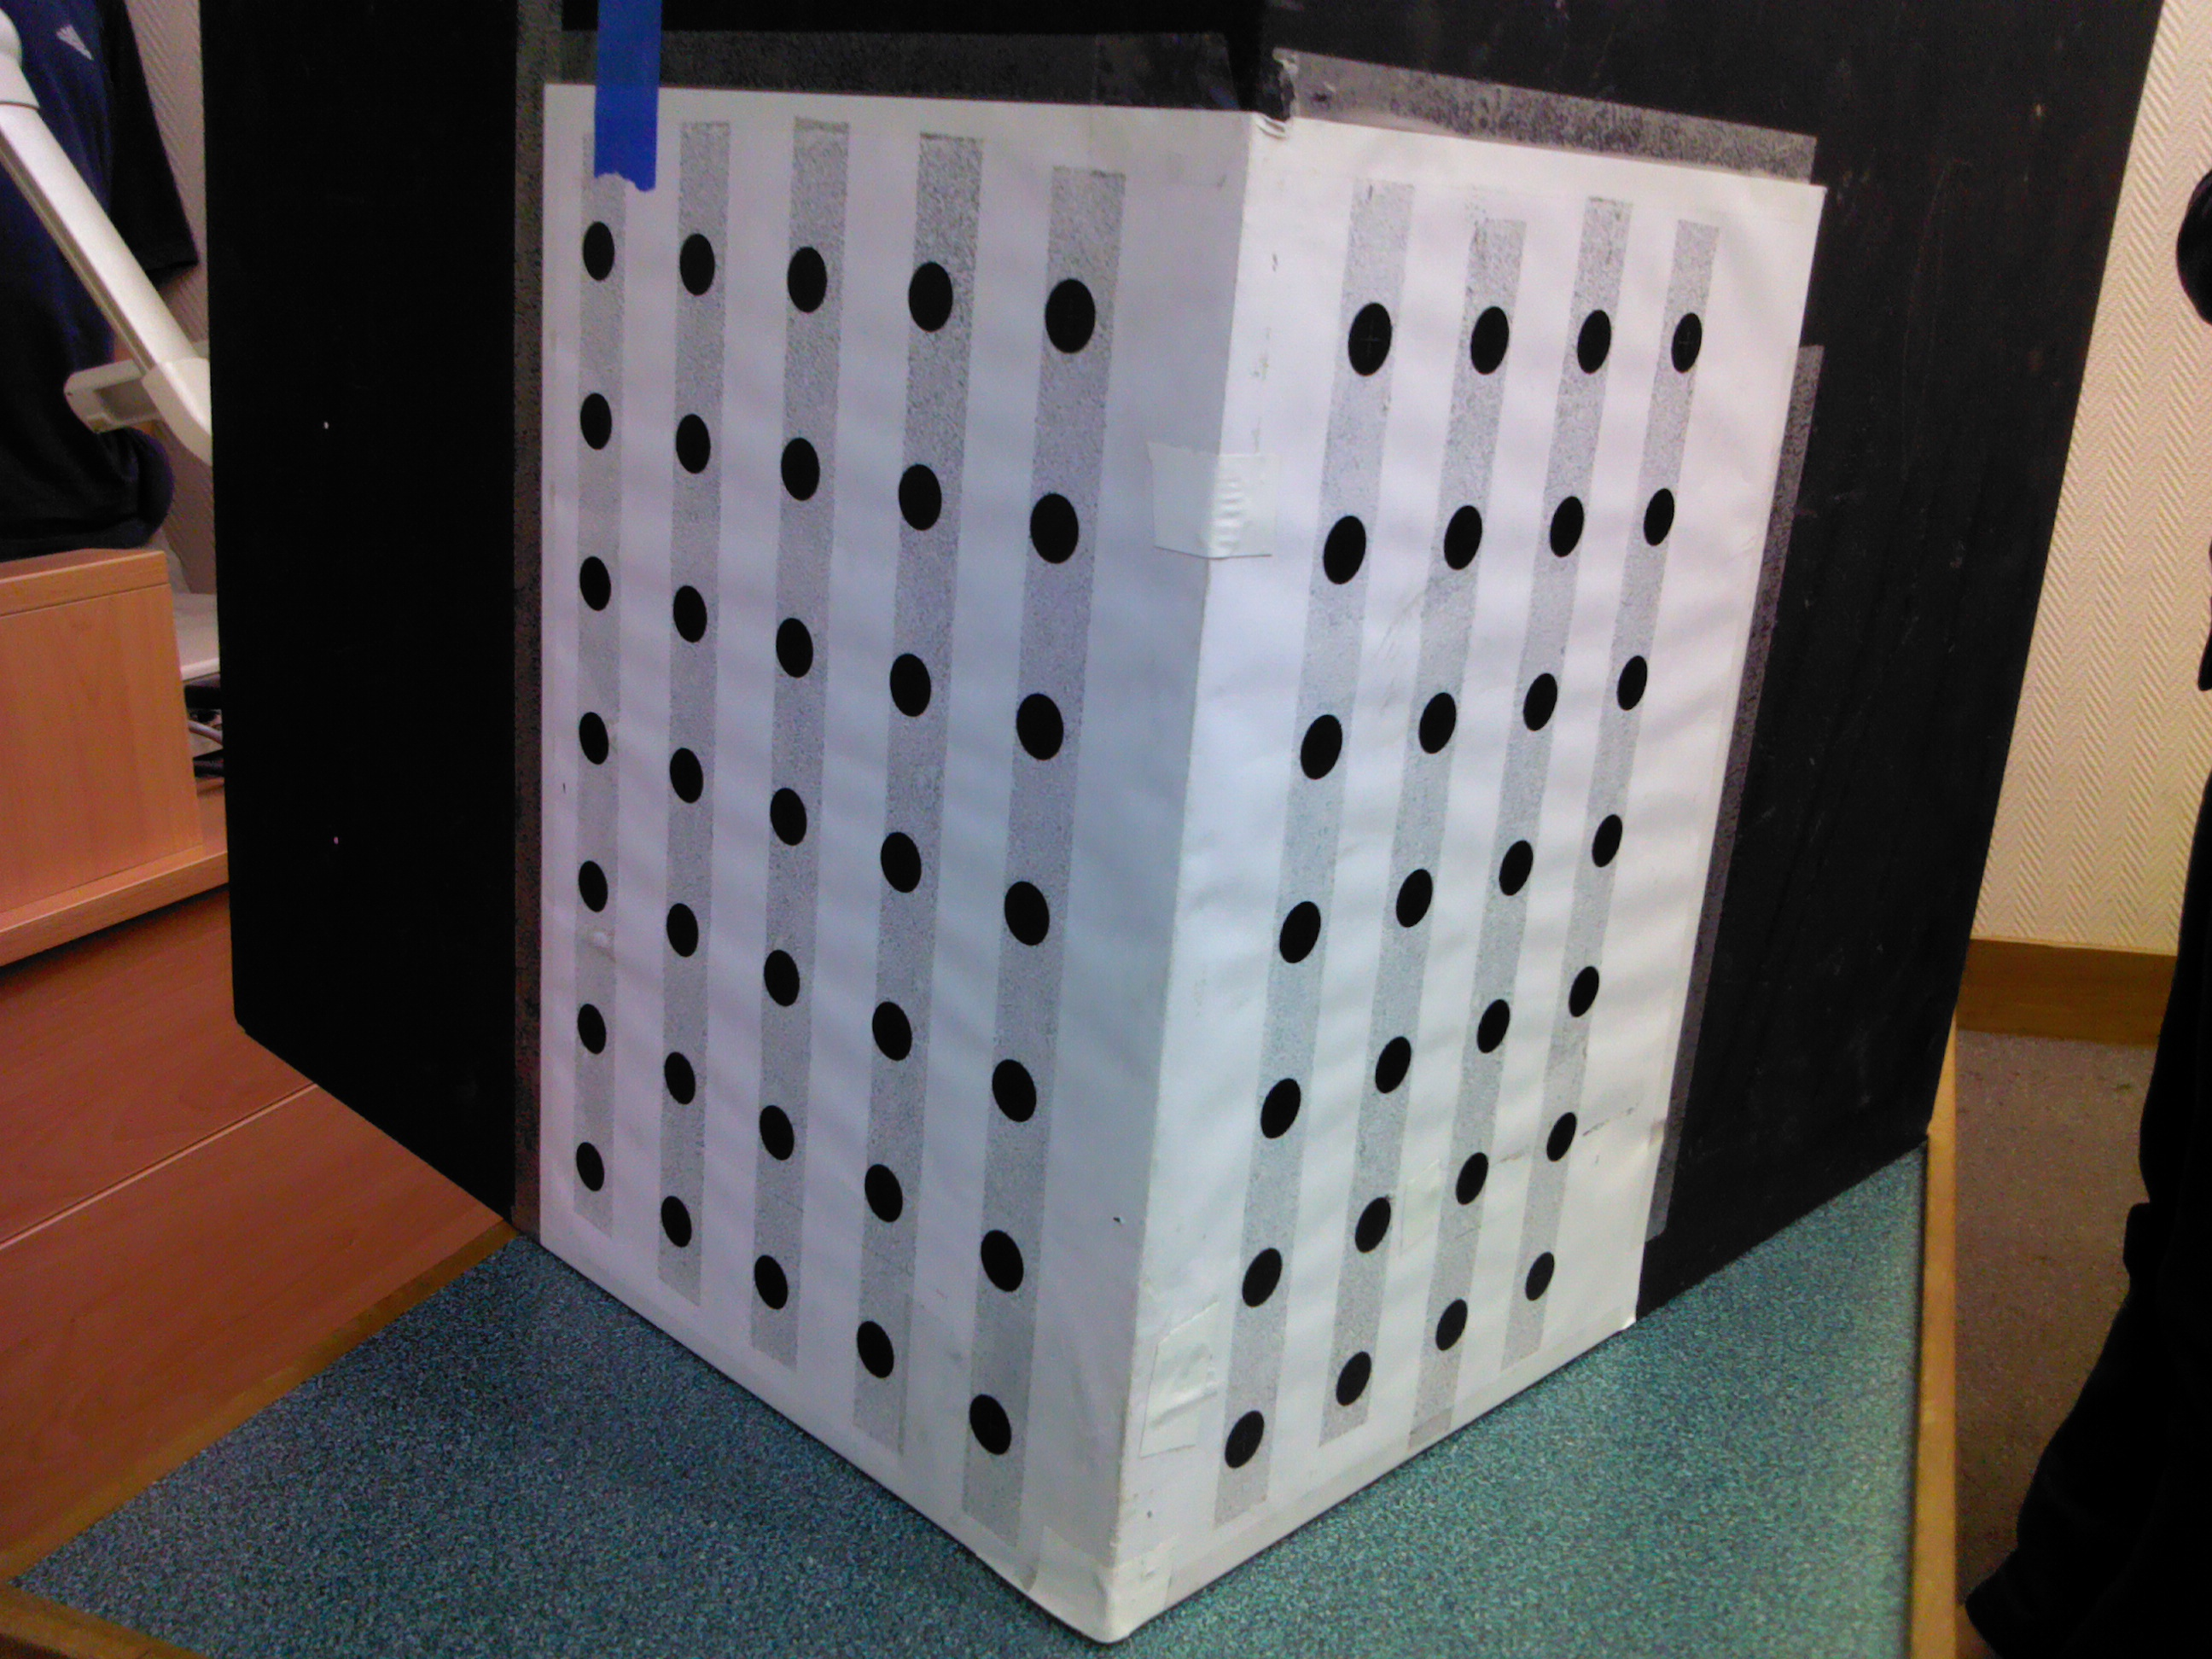
\includegraphics[width=0.6\textwidth]{figures/calibration-object}
  \caption[Calibration object]{Calibration object, demonstrating 35 calibration points on the left face (YZ plane) and 28 on the right face (XZ plane). Calibration points correspond to the centres of the circles. The distance between point centres is 1.5 inches.}
  \label{fig:calib-object}
\end{figure}

\subsubsection{Implementation notes}
Our implementation closely follows the procedure laid out for the monoview non-coplanar case in
\cite{TSAI}. The calibration function derives
the transformation matrix (composed of the rotation matrix, $R$ and
the translation matrix $T$), finds the scale factor $s_x$, and determines the
intrinsic camera values $f$ (focal length) and $\kappa$ (radial
lens distortion parameter). The radial distortion is calculated as far as
$\kappa_1$. The literature suggests that this is sufficient for
reasonably high accuracy using cameras without significant lens
distortion \cite{algebraic-distortion}.

\paragraph{Mapping of image coordinates to world coordinates.}
The world coordinates of the points are measured manually, in units of
inches. These are given as input to the program in the form of a
space-separated text file. The image coordinate points are found by
first running the SURF feature point extraction algorithm described in
section~\ref{sec:features} on the input image, with a relatively high
threshold value (default 500). The feature points detected using this
algorithm are shown to the user on a binary image (obtained using
adaptive thresholding -- see the description of the segmentation
algorithms in section~\ref{sec:segmentation}). The user then has the option
to remove or add points.

The user-corrected points become the input for the second stage of the
calibration algorithm. This stage assumes that there are exactly 63
points selected on the image, and also requires input of exactly
63 3D points (corresponding to the 63 circles on the calibration
object). The image points are first corrected to be closer to the
centre of the circle. This is done by flood filling the binary-thresholded image
from each point with a threshold of 0 (i.e. finding all pixels of the
same colour as the point), and taking the average x and y values from
this region. This means that the user does not have to select points
that are exactly at the centre of the calibration region, but can
click anywhere within it to identify the region.

Following this correction, the image points are mapped to the real
world coordinate points. This is done by a brute-force algorithm
relying on the fact that
\begin{inparaenum}[(a)]
  \item the right and left faces are entirely disjoint in the
    horizontal direction, i.e. no points on the right face have
    x-coordinates lower than any points on the left face, and
  \item the top and bottom outermost points in each face are the
    points closest to the respective image corners on that side of the
    image.
\end{inparaenum}
This algorithm does impose some limitations on the possible viewing
angles of the calibration object. For example, if the image is rotated
sufficiently to make points on the faces overlap in the horizontal direction, the
first assumption breaks down and the image point to world point
mapping will fail.

\paragraph{Back-projection.}
To test the error ratio of the calibration, we reverse the direction
of projection, by projecting the rays from the camera through the
image coordinate points onto the corresponding face planes in world
coordinates (taking into account the (reversed) calibration
parameters). This allows us to measure the distance between these
derived world coordinates and the known ones as an error radius.

\paragraph{Implementation problems.}
We encountered several problems during our implementation. Primarily,
it was not immediately obvious to us that, in going from the coplanar
to the non-coplanar cases, equation (15) in \cite{TSAI} has to be
re-derived from the earlier equation (8b), because it is no longer
true that $z_w=0$. It also proved difficult to get the back-projection
working correctly, due to an earlier confusion about the right-handed nature of the world coordinate system.

\subsubsection{Experimental results}
To test the calibration, we ran the program on four different
pictures of the calibration object: two images taken with two different cameras.
In this section, we go through the results, first by ``sanity
checking" the values from observations of the environment, and then
by looking at the errors from the back-projection estimates.

\begin{table}[htb]
  \centering
  \begin{tabular}{c c c c c c}
    \toprule
    \multicolumn{3}{c}{\textbf{Rotation}} & \multicolumn{3}{c}{\textbf{Translation}}\\
    \midrule
    \multicolumn{3}{c}{$R=\begin{bmatrix}0.69 & -0.72 & 0.08\\
    0.14 & 0.25 & 0.96\\
    -0.70 & -0.65 & 0.28\end{bmatrix}$} &
    \multicolumn{3}{c}{$T=\begin{bmatrix}0.00\\-6.76\\-16.80\end{bmatrix}$} \\
    \midrule
    \multicolumn{2}{c}{\textbf{Scaling}} &
    \multicolumn{2}{c}{\textbf{Focal length}} &
    \multicolumn{2}{c}{\textbf{Distortion}}\\
    \midrule
    \multicolumn{2}{c}{$s_x =0.998$} &
    \multicolumn{2}{c}{$f=-2424.61$} &
    \multicolumn{2}{c}{$\kappa_1=-1.76 \cdot 10^{-8}$}\\
    \bottomrule
  \end{tabular}
  \caption[Calibration results]{Calibration results. This is the
    results of calibration for the first image (labelled 160019 in
    figure~\ref{fig:calib-errors}).}
  \label{tbl:calib-results}
\end{table}

One of the results of the calibration can be seen in
table~\ref{tbl:calib-results}. This is a typical output of the program. First, consider the translation vector. According to the calibration, the corner of the calibration object is
a little less than 17 inches in front of the camera (or camera plane) and slightly less than 7 inches below it. We can tell by observation that these figures are roughly consistent with the
distance from which the picture is taken. Furthermore, table~\ref{tbl:focal-lengths} compares the focal length results for the four images. From this data, it is
apparent that images taken with the same camera have similar focal
lengths, and the focal lengths of images taken with different cameras
are quite different. These two sanity tests together suggest that the calibration has been approximately successful.

\begin{table}[h]
  \centering
  \begin{tabular}{c c}
    \toprule
    \textbf{Image} & \textbf{Focal length}\\
    \midrule
    160019 & -2424.61\\
    160027 & -2412.75\\
    0025 & -4887.01\\
    0026 & -4701.72\\
    \bottomrule
  \end{tabular}
  \caption[Focal length values for the test images]{Abstract focal length
    values for the test images. The images are taken pairwise with two
    different cameras; this is reflected in the focal lengths,
    in that images taken with the same camera have very similar focal
    lengths, and there is a significant variation between the two cameras.}
  \label{tbl:focal-lengths}
\end{table}

To test the error in our calibration values, we 
implemented a back-projection test, as described in the previous
section. From this, we have obtained mean radii of error, i.e. the
distances from the back-projected points to the known locations of the
interest points. These are summarised in
figure~\ref{fig:calib-errors}. The mean errors are roughly four times
the errors Tsai reports in his paper (mean error $0.7$ mm $\simeq0.02$
inches). Note that the fifth column of the figure shows the mean error for one
of the images, using only the eight centre-most calibration points.
This error is not considerably\footnote{ we suspect that it is in fact not \emph{significantly} different, but unfortunately, an oversight during the experimentation process meant we failed to track the data that would allow us to confirm this with a proper statistical model.} different from the case in which all 63 points are used.

An interesting aside: we also tested the camera calibration on the same images with barrel distortion and pincushion distortion artificially introduced, and still reasonable results. We also separated out the "directionality" of the errors, i.e. the overall misplacement of points in the global X, Y and Z directions, and found that the error along the Z axis was considerably less than that along the X and Y axes. For all the tested images and most of their artificially barrel-distorted variants, the error in the X and Y axes was between 2 and 5 times the error in the Z axis.\footnote{ Error became very large in the artificially pincushion-distorted images, so it was difficult to judge the directionality of error in those cases.} This is presumably because the global X and Y axes slope away from the camera position, whereas the global Z axis is (approximately) constant with respect to the camera position.

\begin{figure}[htb]
  \centering
  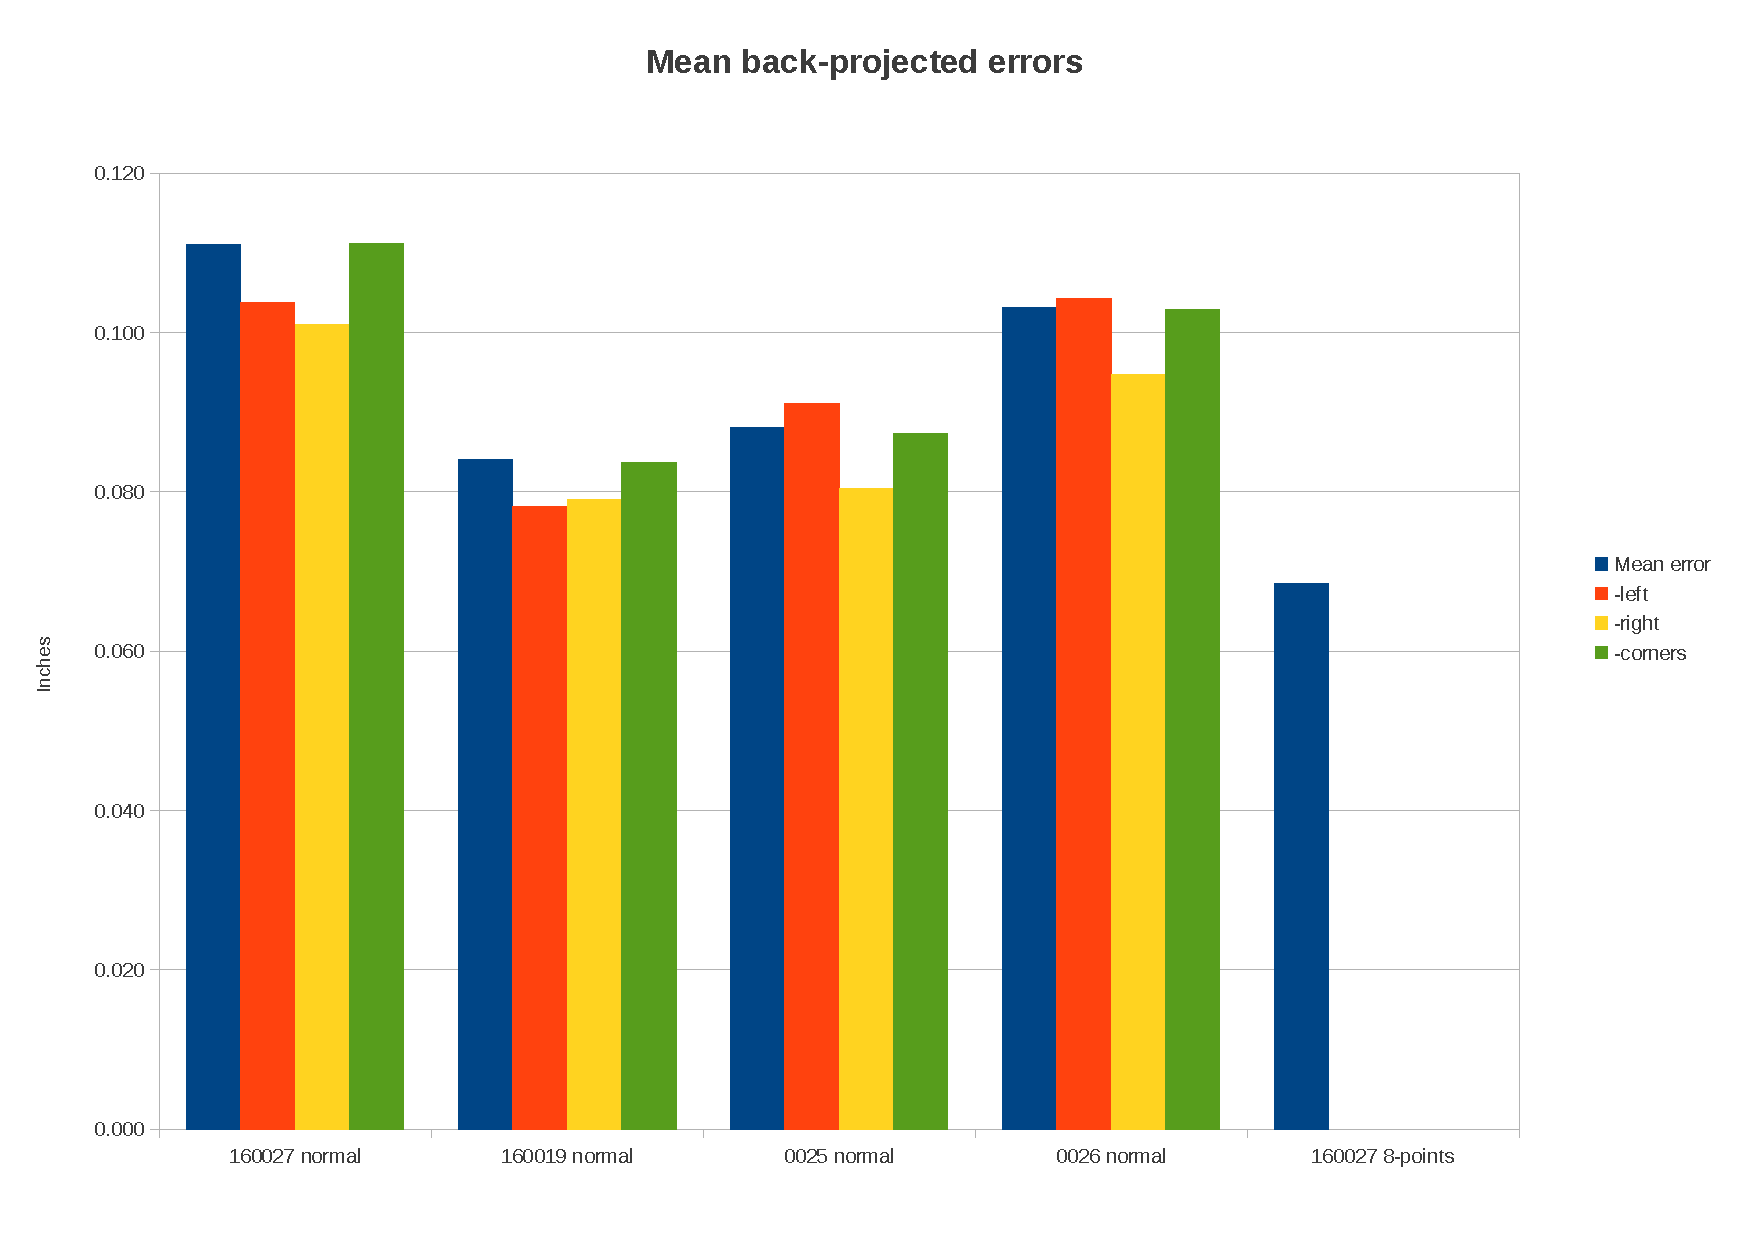
\includegraphics[width=0.75\textwidth]{figures/calibration-means}
  \caption[Mean calibration errors]{Mean calibration errors for all
    calibration points. Each set of bars is from a different image of
    the same calibration object. Two images each are taken with two
    different cameras. The lone bar on the right
    is the mean error calculated from the first image, using only
    the 8 centre-most calibration points.}
  \label{fig:calib-errors}
\end{figure}

\paragraph{Calibration point detection.}
As mentioned, we use our implementation of the SURF feature point extraction algorithm to pick out calibration points from the segmented image. We found this method to work reasonably well. We performed a small test to see how well it identified the 63 calibration points with various thresholds. The results are given in figure~\ref{fig:calib-auto}. The blue bars correspond to true positives, or the number of calibration points successfully identified by the function. The orange bars correspond to false positives, or the number of points of interest returned which did not correspond to calibration points (and would have to be manually removed by the user for the calibration to proceed). The yellow bars correspond to false negatives, or the number of calibration points not identified as points of interest (and would have to be manually added by the user for the calibration to proceed). As we can see from the charts, a threshold of around 500 proves modestly successful at picking out the calibration points.

\begin{figure}[h]
  \centering
  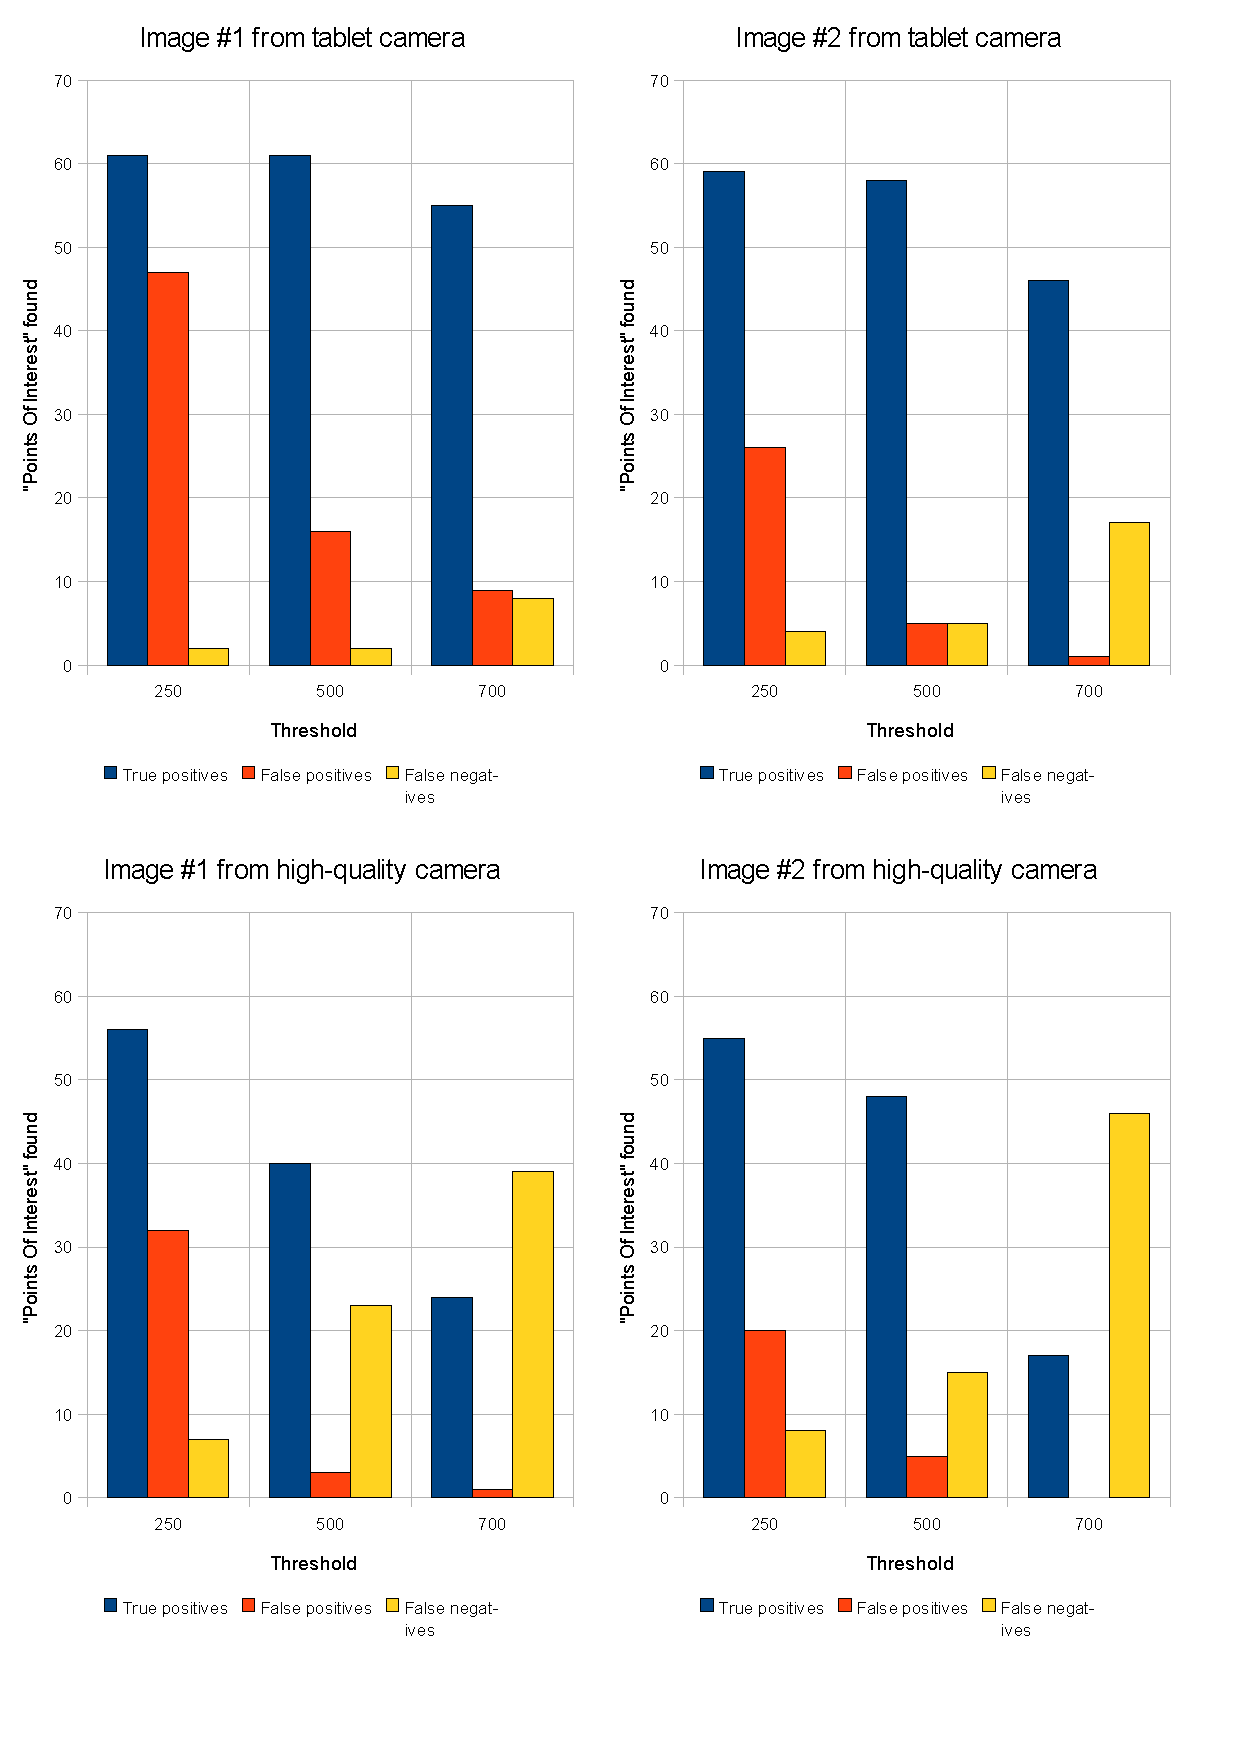
\includegraphics[width=0.7\textwidth]{figures/calibration-auto}
  \caption[Calibration point detection]{Calibration points detected. Each chart is from a different image of
    the same calibration object. The images are taken with two
    different cameras, two with each camera. Each set of bars gives the rate of true positives, false positives and false negatives for a given threshold value.}
  \label{fig:calib-auto}
\end{figure}
